\begin{figure}[h]
    \centering
    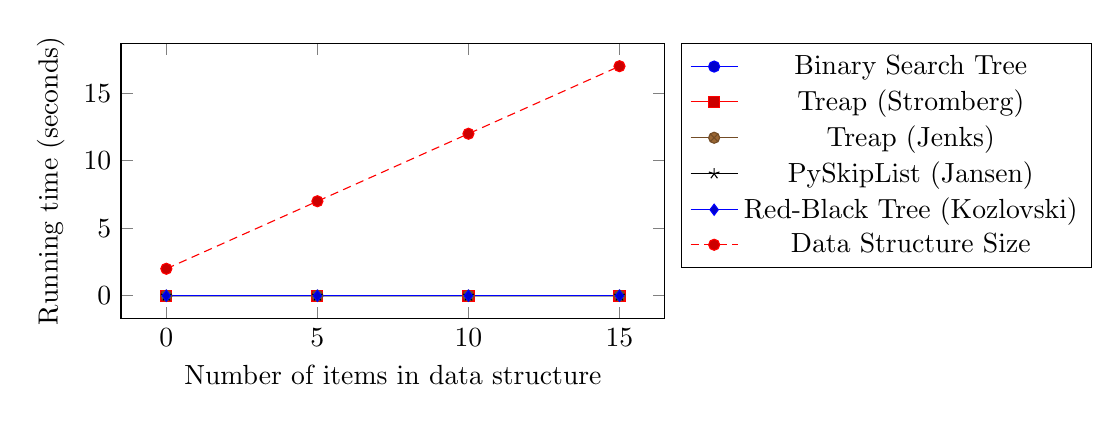
\begin{tikzpicture}
        \begin{axis}[
            xlabel={Number of items in data structure},
            ylabel={Running time (seconds)},
            title={},
            width=0.7\textwidth,
            height=2in,
            legend pos=outer north east
        ]
		\addplot coordinates {
			(0, 3.5137122621027236e-06)
			(5, 3.212536925351235e-06)
			(10, 3.112145146434072e-06)
			(15, 3.112145146434072e-06)
		};
		\addplot coordinates {
			(0, 5.019588945861323e-06)
			(5, 4.618021830192383e-06)
			(10, 3.814887598854501e-06)
			(15, 4.316846493440604e-06)
		};
		\addplot coordinates {
			(0, 3.41332048318585e-06)
			(5, 2.6101862518479687e-06)
			(10, 3.312928704268398e-06)
			(15, 2.7105780307645536e-06)
		};
		\addplot coordinates {
			(0, 1.7568561310513906e-05)
			(5, 1.4054849048411472e-05)
			(10, 1.4857983279749354e-05)
			(15, 1.244858058573571e-05)
		};
		\addplot coordinates {
			(0, 3.2125369253515243e-06)
			(5, 3.41332048318585e-06)
			(10, 3.212536925350946e-06)
			(15, 3.513712262103013e-06)
		};
		\addplot coordinates {
			(0, 2)
			(5, 7)
			(10, 12)
			(15, 17)
		};
        \legend{Binary Search Tree, Treap (Stromberg), Treap (Jenks), PySkipList (Jansen), Red-Black Tree (Kozlovski), Data Structure Size}
        \end{axis}
    \end{tikzpicture}
    \caption{Average of 3 operations, benchmarked every 5, starting at 0.}
\end{figure}